\newpage
\subsection{Flow of Opinion} 
\label{apdx:f1}


\begin{figure}[h]
    \centering
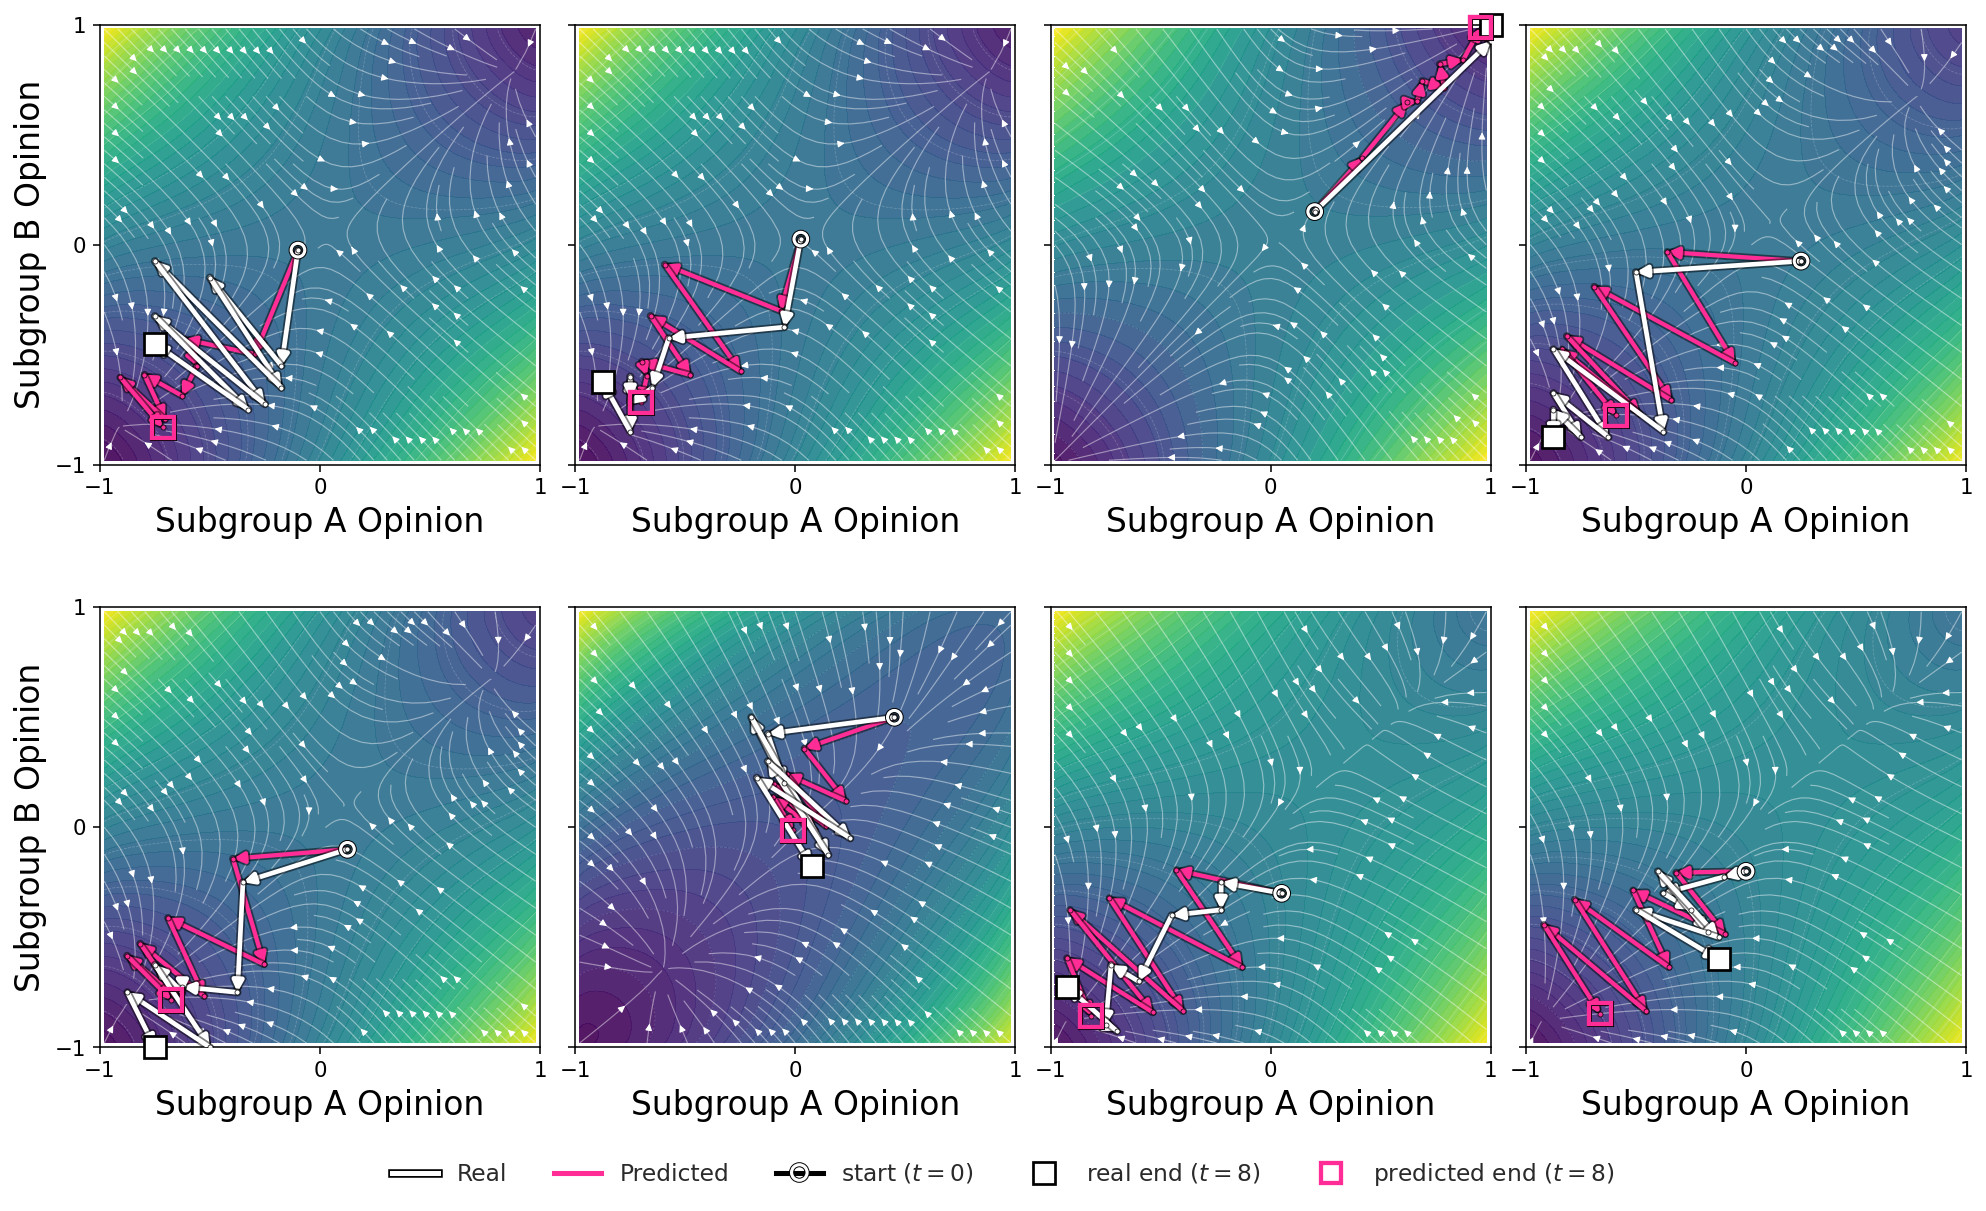
\includegraphics[width=0.99\textwidth]{main/Figures/apx_11_opinion_flow_examples.png}
\caption{\textit{Flow of opinion predicted by the continuous three coupling model.} Each panel is one
group of 32 language-model agents interacting about a question over eight rounds. The axes are the average opinions of the two subgroups. The background shows our fitted model's predictions, with energy represented by colors and the predicted flow (at the continuous time limit) represented by streamlines in the background. White indicates the observed transitions, while pink shows the model's predicted rollout from the initial opinions at $t=0$, that updates the agents synchronously at discrete time intervals $t=1,\dots, T$.  
}
\end{figure}
\begin{figure}[h!]
    \centering
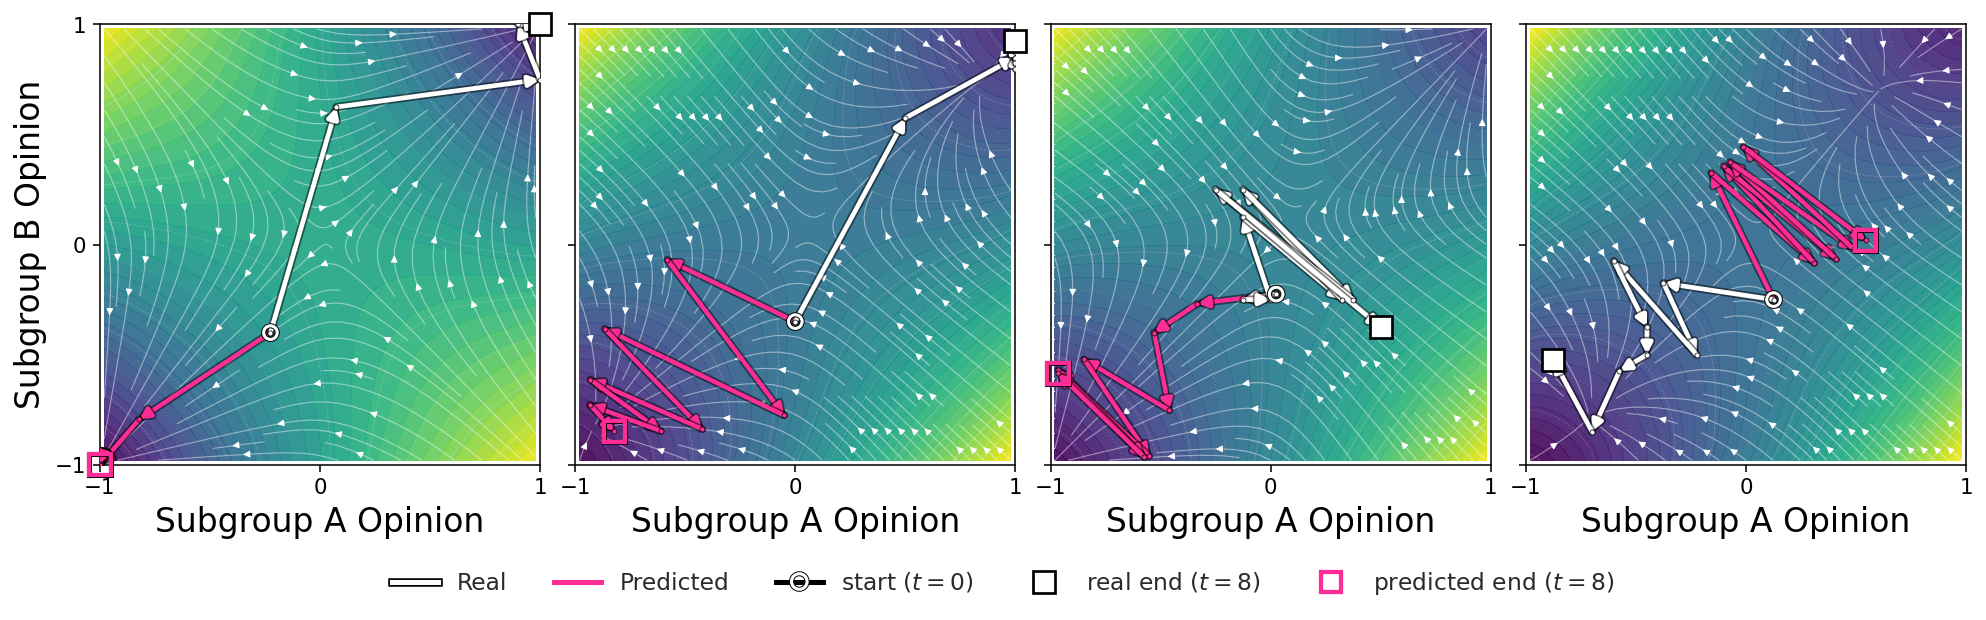
\includegraphics[width=0.99\textwidth]{main/Figures/apx_12_opinion_flow_mismatches.png}
\caption{\textit{Four example group trajectories where predictions do not match the observations.}
}
\end{figure}
\textit{Splitting into groups.} We split the agents into two subgroups based on their opinion at $t=0$. The $N=32$ agents are ranked by their round-0 opinion $\bar{o}_i(0)$; the top half forms group $A$ and the bottom half group $B$, so the two
subgroups always have equal size ($16$ and $16$) and $A$ is by construction the side that starts higher, $n_A(0)\ge n_B(0)$, where $n_A(0)$ denotes the net opinion of the agents in subgroup A. Ties are broken by the following round, then the one after.

At each point on a $220\times220$ grid, we record the net opinions of agents in $A$, $n_A(t)$, and agents in $B$, $n_B(t)$. We generate rollouts and plot the subgroup net opinions at each timestep. The white path shows the real community’s per-round net opinions in the same two-dimensional space, while the pink path shows a rollout from the fitted continuous three-coupling update rule, initialized from the same state. We show selected rollouts on the held-out test set of questions.
